\documentclass[mathserif, 10pt,usenames,dvipsnames]{beamer}

\usepackage{amsmath, mathtools, siunitx}
\usepackage[none]{hyphenat} %removes hyphenation at end of lines
\usepackage{caption}
\usepackage{subcaption}
\usepackage{graphics,graphicx,epsfig,ulem, booktabs} % Makes sure all graphics works
\usepackage{amssymb}
\usepackage{float}
\usepackage{multicol, multirow}
\usepackage{enumitem}
\usepackage{color, soul}
\usepackage{gensymb}
\usepackage{sidecap}
\usepackage{cancel}
\usepackage{wrapfig}
\usepackage{xcolor}
\usepackage{pifont}
%\setlist[itemize]{noitemsep, topsep=-8pt}
\setlist[enumerate]{topsep=-8pt}
\sidecaptionvpos{figure}{c}

\usetheme{Berkeley}
\usecolortheme{beetle}

\newcommand{\labelitemi}{\color{CadetBlue} \ding{228}}
\newcommand{\labelitemii}{\color{CadetBlue} \ding{229}}

\title{Quarkonium}
%\subtitle{Bound States and Phenomena of Mesons}
\author{Matthew Rossetter}
\institute{
    Durham University
}
\date{November 21, 2018}

\begin{document}

\frame{\frametitle{Physics Problem Solving Computing Project} \titlepage}

\begin{frame}
    \frametitle{Introduction}
    \begin{itemize}
        \item Project will solve Schrodinger equation of a quarkonium system
        \item Study the bound states found given by solutions
        \item Expand from this to explore further physics
        \item Quantum Chromodynamics (QCD) is the study the strong force, quarks and gluons
        \item Gluons are the force carriers for the strong force
        \item Quarks cannot exist as free particles
    \end{itemize}
    \begin{center}
        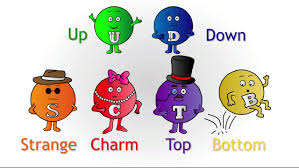
\includegraphics[scale=0.5]{quarks.jpg}
    \end{center}
\end{frame}

\begin{frame}
    \frametitle{Introduction}
    \framesubtitle{Background Physics}
    \begin{itemize}
        \item QCD gets split into two regimes - one can be studied similarly to QED
        \item Charm and Bottom quark systems have high enough masses to be studied using standard methods
        \item A Bottom or Charm quark-antiquark bound pair can be modeled similarly to the hydrogen atom
        \item Apply QCD similarly to QED for hydrogen
        \item The non-relativistic 3D Schrodinger equation is satisfied by these systems
            \begin{align}
                -\frac{\hbar^2}{2\mu}\nabla^2\psi &+ \left[V(r) - E_{nl}\right]\psi = 0 \\
                V(r) &= -\frac{4\alpha_s}{3r} + \beta r
            \end{align}
    \end{itemize}
\end{frame}

\begin{frame}
    \frametitle{Numerical Methods for Solving the Wavefunction}
    \begin{itemize}
        \item Radial wavefunction, $u_{nl}$, found from solving a set of ODEs
            \begin{align}
                \frac{du_{nl}}{dr} &= v_{nl} \\
                \frac{dv_{nl}}{dr} &= \frac{l(l+1)}{r^2}u_{nl} -2\mu(E_{nl} - V(r))u_{nl}
            \end{align}
        \item Solve iteratively to find correct energy
            \begin{itemize}
                \item Guess three initial energies/betas and solve equation
                \item Compare nodes and turning points of solution and theory
%                    \begin{gather}
%                        \text{Turning points} = n-l \\
%                        \text{Nodes} = n-l-1
%                    \end{gather}
                \item Narrow down energies/betas until a solution is found
                \item Guess new inital energies if no solutions found
                \item Use Simpsons method, or similar numerical integrator, to normalise solution
            \end{itemize}
    \end{itemize}
\end{frame}

\begin{frame}
    \frametitle{The Milestone Project}
    \framesubtitle{Solving the Hydrogen Wavefunction}
    \begin{columns}[c]
        \column{0.5\textwidth}
        \begin{center}
            \includegraphics[scale=0.2]{images/hydro.png}
        \end{center}
        \begin{itemize}
            \item Program for Quarkonium applied to Hydrogen
            \item $\frac{4\alpha_s}{3} \to \frac{1}{137}, \beta \to 0, \mu \to m_e$
            \item Iterate over energies
        \end{itemize}
        \column{0.5\textwidth}
        \begin{itemize}
            \item $E_{1,0} = -13.6\,$eV
            \item $E_{2,0} = -3.39\,$eV
            \item $E_{2,1} = -3.25\,$eV
        \end{itemize}
        \begin{center}
            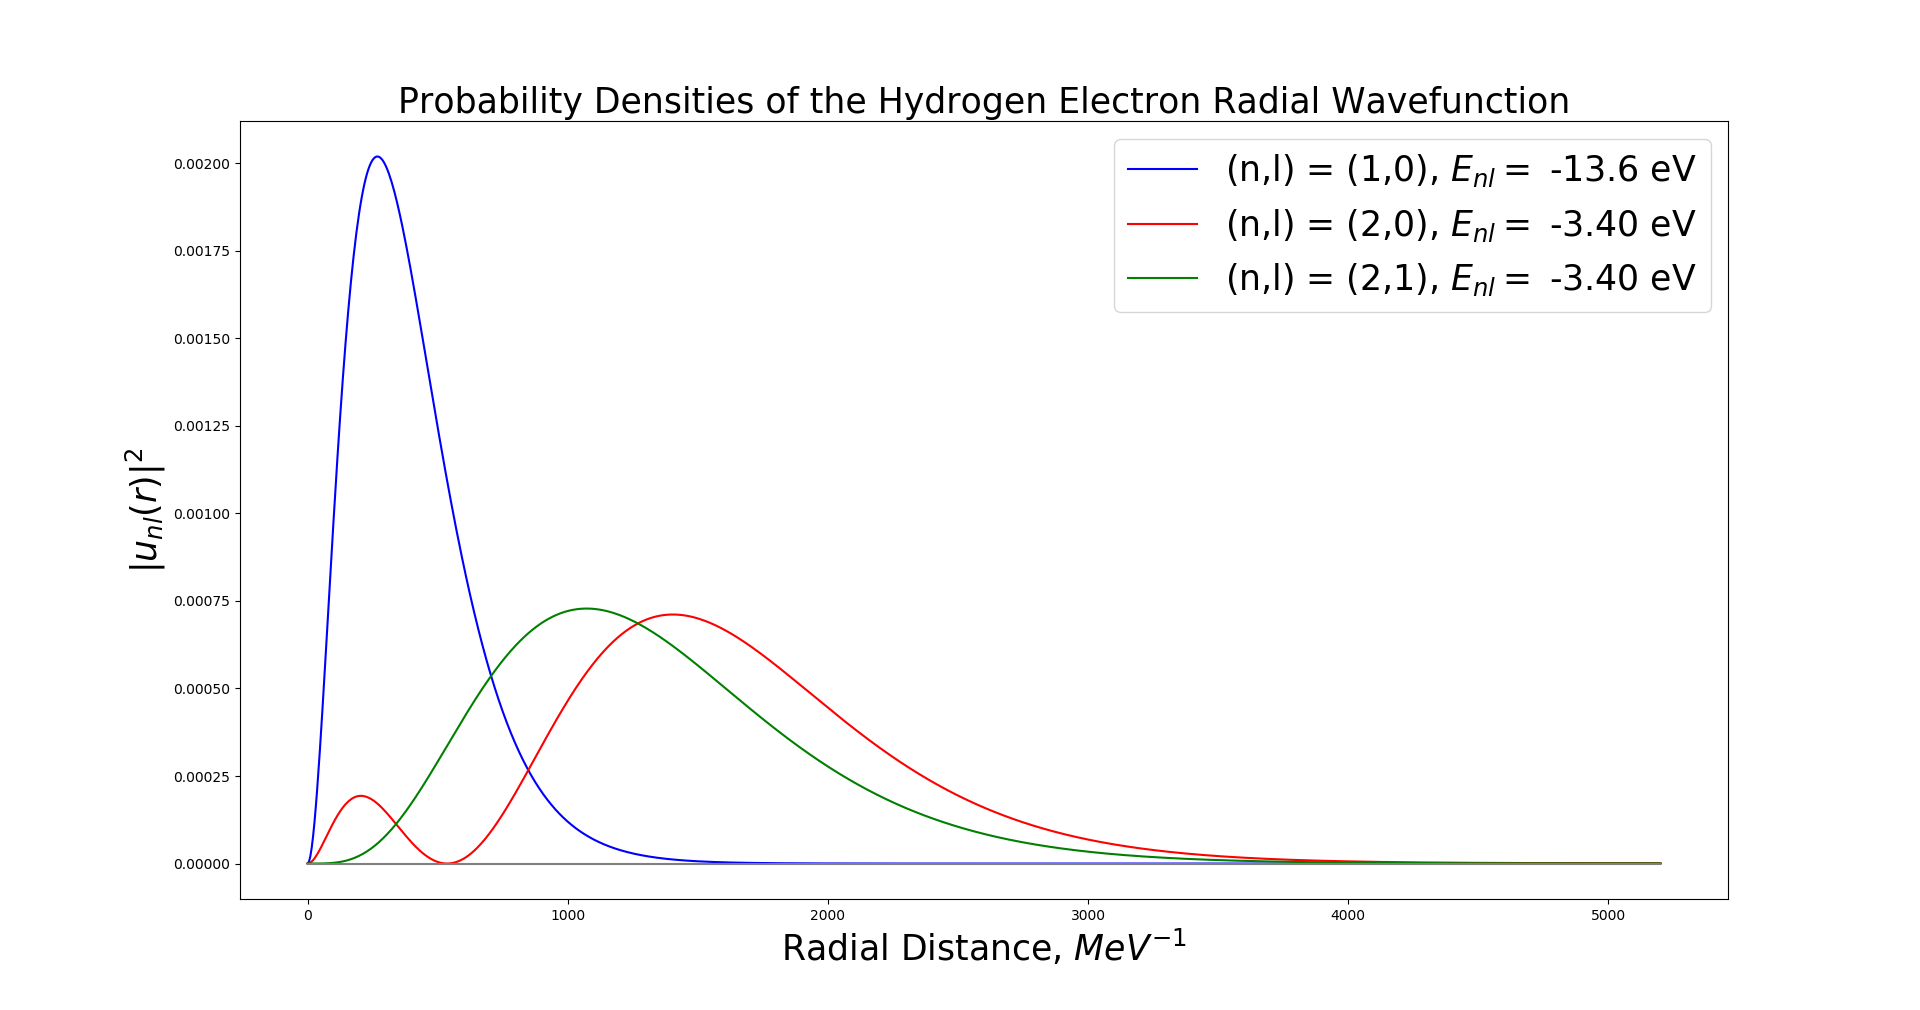
\includegraphics[scale=0.2]{images/probs.png}
        \end{center}
        \end{columns}
\end{frame}

\begin{frame}
    \frametitle{Further Extensions}
    \begin{itemize}
        \item Will apply program to charmonium and bottomonium
        \item Possible ventures:
            \begin{itemize}
                \item Consider other models of the potential
                \item Use program to solve and study other quark systems
                \item Time dependence of states and lifetime
                \item Hyperfine splitting and transition between spin states 
                \item Charmonium melting into quark-gluon plasma
            \end{itemize}
    \end{itemize}
    \vspace{-20pt}
    \begin{columns}[c]
        \column{0.5\textwidth}
        \begin{center}
            \begin{figure}[H]
                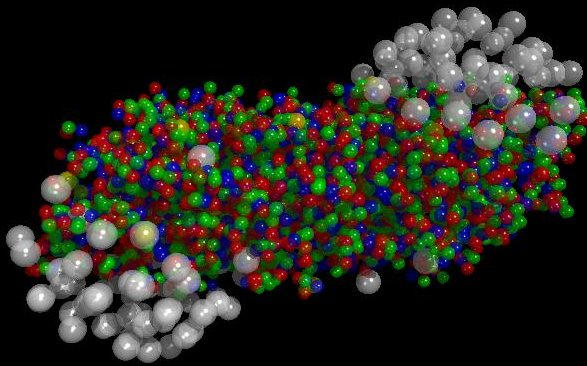
\includegraphics[scale=0.3]{QGM.jpeg}
                \caption{\footnotesize Quark-Gluon Plasma}
            \end{figure}
        \end{center}
        \column{0.5\textwidth}
        \begin{center}
            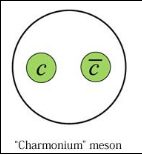
\includegraphics[scale=0.35]{charm.png} \\
            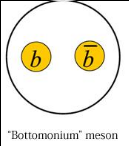
\includegraphics[scale=0.35]{btm.png}
        \end{center}
    \end{columns}
\end{frame}

\end{document}
